\documentclass[a4paper,11pt]{scrreprt}
    %% Used for changing geometry of the page
    %% Cover page text cannot overlay cover sketching/style 
    %% https://ctan.org/pkg/geometry?lang=en
\usepackage{geometry}
\geometry{
    top=30pt
}
    %% Changes language of some packages protocols
    %% e.g., when captioning images: Figure 1. -> Figura 1.
    %% https://ctan.org/pkg/babel?lang=en
\usepackage[portuguese]{babel}
    %% Used for special fonts
    %% Cannot be compiled with pdflatex
    %% https://ctan.org/pkg/fontspec?lang=en
\usepackage{fontspec}
    %% Arial FONT
    \setmainfont{Arial}
\usepackage{subfiles}
    %% More colors and color options
    %% https://ctan.org/pkg/xcolor?lang=en
    %% https://ctan.org/pkg/colortbl?lang=en
\usepackage{xcolor,colortbl}
    %% More tabular options, like dashed/dotted lines
    %% https://ctan.org/pkg/arydshln?lang=en
\usepackage{arydshln}
    %% List of acronyms
    %% https://ctan.org/pkg/nomencl?lang=en
\usepackage[intoc]{nomencl}
    %% Must be called to init nomencl environment  
    \makenomenclature
    %% More images options/settings
    %% https://ctan.org/pkg/graphicx?lang=en
\usepackage{graphics}
    %% Defining subdirectories to image path enviornment
    %% \graphicspath{{sub1}{sub2}...{subN}}
    \graphicspath{{images}}
    
    %% used to handle cross-referencing commands in LaTeX to produce hypertext links in the document
    %% https://ctan.org/pkg/hyperref?lang=en
\usepackage{hyperref}
    %% math environments
    %% https://ctan.org/pkg/amsmath?lang=en

    %% settings
    \hypersetup{
        colorlinks,
        citecolor=black,
        filecolor=black,
        linkcolor=black,
        urlcolor=black
    }

\usepackage[backend=bibtex, style=numeric-comp]{biblatex}
\addbibresource{biblio.bib}

\usepackage{amsmath}
    %% Defining backgrouns, used to make the cover
    %% https://ctan.org/pkg/background?lang=en
\usepackage[some]{background}
    %% Used to make drawings or complex graphics
    %% http://pgf.sourceforge.net/pgf_CVS.pdf
\usepackage{tikz}
    %% Tikz library to point operations ((x1,y1) + (x2,y2))
    \usetikzlibrary{calc}
\usepackage{lscape}
%% Defining sfdefault font and default font for document
\renewcommand{\familydefault}{\sfdefault}

\usepackage{float}

\usepackage{minted}

%% Costume made cover 
%% From there you can use \makecover command to build the cover
%% Blue cover color
\definecolor{titlepagecolor}{RGB}{54,95,145}

%==========================================================================
% COLORED BAR ON THE LEFT SIDE
%==========================================================================

\backgroundsetup{
    scale=1,
    angle=0,
    opacity=1,
    contents={
            \begin{tikzpicture}[remember picture,overlay]
                \path [fill=titlepagecolor]
                (current page.north west) -- ($(current page.north west) + (5,0)$)
                -- ($(current page.south west) + (5,0)$)-- (current page.south west);
                \node[color=white] at ($(current page.south west) + (3,4)$) {\bfseries {\fontsize{50}{60} \textsf{SD}}};
                %\node[color=titlepagecolor] at ($(current page.south west) + (5.8,4)$) {\bfseries {\fontsize{120}{60} \textsf{4}}};
            \end{tikzpicture}
        }
}

%==========================================================================
% TITLE PAGE INFO
%==========================================================================

%% Changes values in this field to show information in the cover and back cover about your team/project


%% TITLE
\title{Sistema de gestão de reservas de voos}

%% AUTHORS
\author{
    \begin{tabular} { c c }
        
\includegraphics[scale=0.2]{author/marco.jpg} & 
\includegraphics[scale=0.2]{author/mariana.jpg} \\
        62608 - Marco Sousa                           & 93198 - Mariana Marques                       \\
        %\hline                                                                                        \\
        
\includegraphics[scale=0.2]{author/ze.jpg} & 
\includegraphics[scale=0.2]{author/miguel.jpg} \\
        93271 - José Malheiro                         & 94269 - Miguel Fernandes
    \end{tabular}
}

%% Date

\date{\today}

%% Course
\newcommand{\Course}{Licenciatura em Engenharia Informática}

%% Department
\newcommand{\Department}{Escola de Engenharia}

%% UniName
\newcommand{\UniName}{Universidade do Minho}

\newcommand{\UcName}{Sistemas Distribuídos}

\newcommand{\GroupId}{Grupo 12}

%% UniPic
\newcommand{\UniPic}{
\includegraphics[scale=0.09]{uminho.png}}

%% University 
\newcommand{\University}{
    \begin{flushleft}
        \UniPic
    \end{flushleft}
    \textcolor{gray}{\small\textbf{\textsf{\UniName}}}\par
    \textcolor{gray!80!white}{\small{\textsf{\Department}}}\par
    \textcolor{gray!70!white}{\small{\textsf{\Course}}}
}

%% UC
\newcommand{\UC}{
    \begin{flushleft}
        \par\textcolor{titlepagecolor}{  \LARGE\textbf{\textsf{Unidade Curricular de \\ \UcName}}}
    \end{flushleft}
}

%% School Year
\newcommand{\SchoolYear}{
    \small{\textsf{Ano Letivo de 2021/2022}}}


%% Define new command to show title, author and date
\makeatletter
\let\Title\@title
\let\Author\@author
\let\Date\@date
\makeatother

%==========================================================================
% CLASSIFICATION SECTION 
%==========================================================================

%% School Year
\newcommand{\ReceptionDate}{}
%% Responsible
\newcommand{\Responsible}{}
%% Evaluation
\newcommand{\Evaluation}{}
%% Observations
\newcommand{\Observations}{}


%% MAKETEMPLATE
\newcommand{\makecover}{

    %==========================================================================
    % BEGIN COVER PAGE 
    %==========================================================================

    %% Removes page number on footer
    \thispagestyle{empty}

    %% No indentation 
    \setlength{\parindent}{0em}

    %% Put Background defined on \backgroundsetup, in this page
    \BgThispage

    %% Changing geometry to prevent overlay with text
    %% At the end of back cover, geometry is default with \restoregeometry
    \newgeometry{top=3.5cm,left=6cm,right=3cm,bottom=2cm}

    %% builds university info defined previously
    \University
    \vspace{1cm}
    %% builds curricular unity info defined previously
    \UC
    %% builds school year info defined previously
    \SchoolYear

    \vspace*{4cm}
    %% bigger space (i think its the default one) between paragraphs 
    \setlength{\parskip}{1em}

    %% builds title info defined previously
    \par\textbf{\textsf{\huge\Title}}
    \par\textbf{\GroupId}
    \vspace{1cm}
    %% builds author(s) info defined previously
    \par\begin{center}
        \Author
    \end{center}

    \vspace{0.5cm}

    %% builds date info defined previously
    \par\Date
    \restoregeometry
    \pagebreak

    %==========================================================================
    % END COVER PAGE 
    %==========================================================================
}


\graphicspath{ {./assets/} }

\begin{document}

\pagenumbering{gobble}

% builds the cover
\makecover

%==========================================================================
% BEGIN ABSTRACT PAGE
%==========================================================================

%% Abstract name: \Large font size, flushed left and paragraph skip before abstract content

\renewenvironment{abstract}
{\par\noindent\textbf{\Large\abstractname}\par\bigskip}
{}

\begin{flushleft}
    \begin{abstract}
        %=============
        % How to build an abstract
        % https://users.ece.cmu.edu/~koopman/essays/abstract.html
        %=============
        A crescente procura por serviços cliente - servidor, obrigada a que um sistema seja capaz
        de responder a múltiplos pedidos de forma concorrente.
        Como consequência, surge a necessidade de moldar o sistema para que este tenha um comportamento
        determinístico, independentemente da circunstância de utilização.
        Assim, na sequência da Unidade Curricular de \textbf{Sistemas Distribuídos}, surge a oportunidade
        de desenvolver uma aplicação com múltiplos clientes e um servidor, ambos \textit{multi-threaded}.
        
        O projeto proposto corresponde a um sistema de reservas de voos, denominado \textit{Flight Manager}.
        Este, conforme referido, será capaz de ter um servidor que responde a múltiplos clientes, de forma
        concorrente.
        A linguagem de programação utilização foi \textbf{\textit{Java}}, com recurso a \textit{Socket} TCP
        para efetuar a comunicação entre cliente-servidor.
        
        \par \textbf{Área de Aplicação}: Sistemas Distribuídos
        \par \textbf{Palavras-Chave}: Sistemas Distribuídos, \textit{Threads}, \textit{Multithreaded}, 
        \textit{Middleware}, Servidor, Cliente, Serialização, \textit{Data Transfer Object},
        \textit{Sockets}, TCP, \textit{Tagged Connection}
    \end{abstract}
\end{flushleft}

\pagebreak

%==========================================================================
% END ABSTRACT PAGE 
%==========================================================================

%==========================================================================
% BEGIN INTRODUCTION
%==========================================================================

%% Starting page numbering here
\pagenumbering{arabic}

\chapter{Introdução}

O presente relatório foi escrito no âmbito da Unidade Curricular de Sistemas Distribuídos (SD), sendo o
tendo como principal objetivo apresentar uma possível solução para um Sistema de Gestão de Reservas,
que iremos designar \textit{Flight Manager}, capaz de responder às funcionalidades propostas pela equipa docente.

Assim, será apresentado um sistema \textit{cliente-servidor} que, do lado do servidor,
será capaz de atender múltiplos clientes e, do lado do cliente, será capaz de comunicar com o servidor
e executar métodos assíncronos e síncronos.

Para dar resposta ao proposto, utilizou-se um componente comum a ambos os sistemas, um \textbf{Middleware},
que servirá de ponte de ligação entre os \textit{hosts}.
O objeto de comunicação, será um \textit{Data Transfer Object} e, a partir deste, será derivado
múltiplos objetos relacionados com pedidos e respostas.

Com o desenvolvimento deste projeto, pretende-se apromirar vários conceitos de Sistemas Distribuídos,
tais como:
\begin{itemize}
    \item Programação com \textit{Sockets}
    \item Programação com múltiplas \textit{Threads} (\textit{MultiThread})
    \item Programação Concorrente (estado partilhado)
    \item Exclusão Mútua
    \item Serialização de Objetos
    \item Arquitetura Cliente-Servidor
    \item Desenvolvimento de \textit{Middleware}
\end{itemize}

%==========================================================================
% END INTRODUCTION
%==========================================================================

\chapter{Análise de Requisitos} \label{chap:analise_requisitos}

O enunciado proposto, remete à conceção e implementação de uma plataforma para gestão de reservas 
de voos, apresentando um conjunto de requisitos funcionais que o sistema deve responder.

A partir do enunciado, identificou-se dois tipos de utilizadores: cliente e adminstrador.
Cada um terá um conjunto de funcionalidades associadas,
tendo sido captadas num Diagrama de Use Case (ver \ref{img:use_case}).

Assim, a nível estrutural, definiu-se três componentes principais:
\begin{itemize}
    \item[\textbf{Cliente}] Interface de interação com o utilizador para utilizar as funcionalidades definidas
    \item[\textbf{Middleware}] Ponte de comunicação entre o cliente e o servidor
    \item[\textbf{Servidor}] Responsável pelo tratamento dos pedidos do cliente
\end{itemize}

Definida a estrutura e as funcionalidades, passou-se para a modelação comportamental do sistema.

\section{Modelação Comportamental} \label{strat_esc}

Por forma a permitir uma implementação sustentada, optou-se por efetuar a modelação comportamental 
do sistema.
Para isso, começou-se por definir a forma como o cliente e o servidor iriam comunicar.
Esta revelou-se como uma das etapas fundamentais para o funcionamento da aplicação,
tendo como perspetiva a sua escalabilidade e manutenção.

\subsection{Comunicação}

A troca de mensagens entre o cliente e o servidor será mediada por um \textbf{Middleware} (ver \ref{img:middleware}).
Pode-se encontrar um esboço da estratégia analisando o diagrama \ref{img:comunicacao}.

\subsubsection{Middleware}

No \textit{middleware} (ver \ref{img:middleware}), haverá especialização do lado do cliente, por forma a receber respostas e enviar pedidos e
do lado do servidor, para receber pedidos e enviar respostas.
Esta especialização, serve apenas para facilitar a implementação, pois, na realidade, o objeto de comunicação
será sempre o mesmo: uma \mintinline{java}{Frame} que terá no seu corpo informação sobre o pedido, nomeadamente
uma \textit{tag} que a identifica e um \textit{Data Transfer Object} (DTO).
Este último, será um dos principais atores na troca de informação, pois a partir da sua especialização,
será possível criar cada um dos pedidos e cada uma das respostas, conforme o conteúdo necessário.
Com o objetivo de generalização do código, colocou-se que a classe \textit{DTO} será abstrata e terá como método,
também este abstrato, a serialização (\textit{serialize}).

\subsection{Servidor}
Dotado de um \textit{ServerSocket}, este será capaz de estabelecer ligação com cada cliente,
sendo-lhe atribuída uma \textit{Thread} própria, partilhando um estado comum com arquitetura \textbf{Facade}: 
\mintinline{java}{IFlightManager} (ver \ref{img:flight_manager}).
Neste, poderá identificar-se dois subsistemas: \textit{Booking Manager} e \textit{User Manager}.

Utilizou-se os princípios \textit{SOLID} \cite{wiki:solid} ao longo da implementação de todo o código,
assim como o seu planeamento.

\subsubsection{BookingManager}


De modo a ter um desenvolvimento mais estruturado, aplicando recursos disponibilizados através de outras 
Unidades Curriculares, foram previamente construídos diagramas para os principais elementos do sistema.

A partir das funcionalidades mencionadas no enunciado do trabalho proposto, foram distribuídas as opções para os
utilizadores da aplicação, seguindo a conceção do sistema.

Esta, divide-se em três grandes componentes:
\begin{itemize}
    \item[Cliente]{Responsável pela apresentação e envio dos pedidos disponíveis do Cliente.}
    \item[Servidor]{Responsável pela resposta por parte do Servidor.}
    \item[Middleware]{Construtor das \textit{Querys} e \textit{Responses}, bem como gere o suporte para a conexão.}
\end{itemize}

Considerou-se mais intuitivo previamente apresentar o modo como a conexão do Servidor/Cliente é geridas e o tipo
de mensagens criadas, sendo a primeira grande componente da aplicação a ser apresentada o: \textit{Middleware}.

\subsection{Middleware}
\subfile{middleware.tex}

\section{Cliente}
\subfile{cliente.tex}

\section{Servidor}
\subfile{servidor.tex}

\section{Funcionalidades Adicionais}

No seguimento da realização das funcionalidade obrigatórias pré-definidas pela equipa docente, 
foi considerada a adição de aspetos adicionais, de modo a enriquecer a resposta previamente 
construída.

\chapter{Considerações Finais}
\section{Conclusões}

Ao longo do desenvolvimento do projeto, e com o auxilio da equipa docente para qualquer questão 
relativa à matéria lecionada e à conceção do trabalho, o grupo foi munido com todos os conceitos
e materiais necessários para o bom desenvolvimento do sistema, \textit{Flight Manager}.

A partir de conceitos de outras unidades curriculares, o grupo foi possibilitado a resolver uma 
solução outrora complexa, a partir de um estruturamento planificado e modelado, usando para tal 
o sistema de modelação \textit{Visual Paradigm}.
Este permitiu, muito mais facilmente, fragmentar o que era necessário resolver para colocar o 
sistema a correr, poupando muito tempo que podia ser perdido, ao construir a aplicação "à mediada
que fazia".

O grupo encontra-se orgulhoso por poder implementar um sistema que não só responde às funcionalidades 
básicas estabelcidades pela equipa docente, com uma plataforma bem construída do ponto de vista
de encapsulamento e organização dos vários constituintes.

Escusado é dizer que muniu todos os participantes com experiência na realização de projetos que sigam 
os conceitos de \textbf{Sistemas Operativos}, nomeadamente a exclusão mútua, a programação com \textit{sockets} e
com várias \textit{Threads}.

\section{Trabalho Futuro}

Apesar de todo o processo de desenvolvimento do sistema \textit{Flight Manager} ter coincidido com as espectativas
colocadas pelo grupo, e, até permitido adicionar funcionalidades numa tentativa de obter um melhor aproveitamento,
existem alguns pontos que poderiam ser abordados numa iteração seguinte do \textbf{Flight Manager}.

Como qualquer sistema que visa a interação com utilizadores sem conhecimentos dentro da área de informática, o 
manuseamento de um terminal para utilizar a plataforma pode tornar-se incómodo.
Dado a aplicação querer satisfazer as necessidades de utilizadores comuns, seria de extrema importância a conceção
de uma interface com o utilizador intuitiva e simples de usar.
Assim, um dos problemas seria a criação de uma \textit{framework} conceptual para o \textbf{Flight Manager}.

Outra equívoco seria a adição de mais funcionalidades. 
O aperfeiçoamento da aplicação, de modo a chegar a um estado competitivo para o mercado atual, passaria pela
implementação de várias e diferentes funcionalidades que o distingue dos restantes produtos análogos.


\printbibliography
%==========================================================================
% BEGIN LISTA DE SIGLAS E ACRÓNIMOS
%==========================================================================

%% Portuguese babel does not translate this environment
\renewcommand{\nomname}{Lista de Siglas e Acrónimos}

%% Text that can be shown before acronyms list
\renewcommand{\nompreamble}{}

%% acronyms
\nomenclature[01]{\textbf{SD}}{Sistemas Distribuídos}
\nomenclature[02]{\textbf{DTO}}{\textit{Data-Transfer Object}}
\nomenclature[03]{\textbf{UC}}{Unidade Curricular}
\nomenclature[04]{\textbf{plataforma}}{Sistema de gestão de reservas de voos}
\nomenclature[05]{\textbf{sistema}}{Sistema de gestão de reservas de voos}
\nomenclature[06]{\textbf{aplicação}}{Sistema de gestão de reservas de voos}
\nomenclature[06]{\textbf{programa}}{Sistema de gestão de reservas de voos}

%% Show acronyms
\printnomenclature

%==========================================================================
% END LISTA DE SIGLAS E ACRÓNIMOS
%==========================================================================

%==========================================================================
% BEGIN ANEXOS
%==========================================================================

\addchap{Anexos}
\addsec{Anexo 1 - Diagrama de Use Case}
\begin{figure}[!ht]
    \centering
    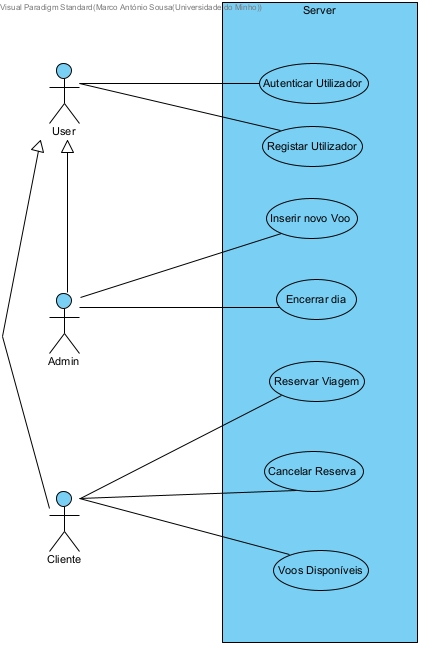
\includegraphics[width=0.8\linewidth]{diagramas/useCaseDiagram.jpg}
    \caption{Diagrama de Use Case} \label{img:use_case}
\end{figure}

\addsec{Anexo 2 - Diagrama de Comunicação}
\begin{figure}[!ht]
    \centering
    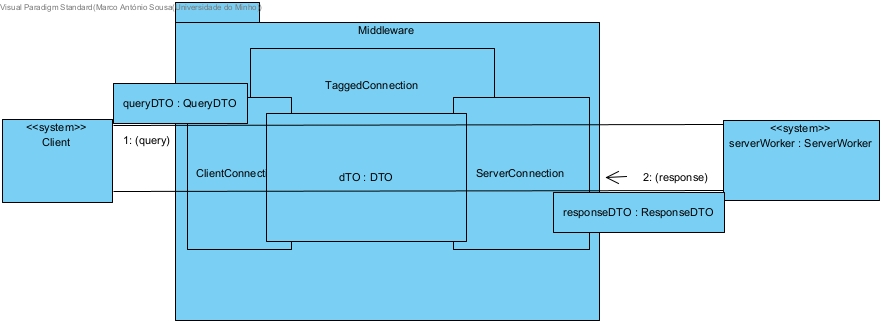
\includegraphics[width=\linewidth]{diagramas/MiddlewareCommunicationDiagram.jpg}
    \caption{Diagrama de Comunicação - versão $\beta$} \label{img:comunicacao}
\end{figure}

\begin{landscape}
\addsec{Anexo 3 - Diagrama de Classes do Middleware}
\begin{figure}[!ht]
    \centering
    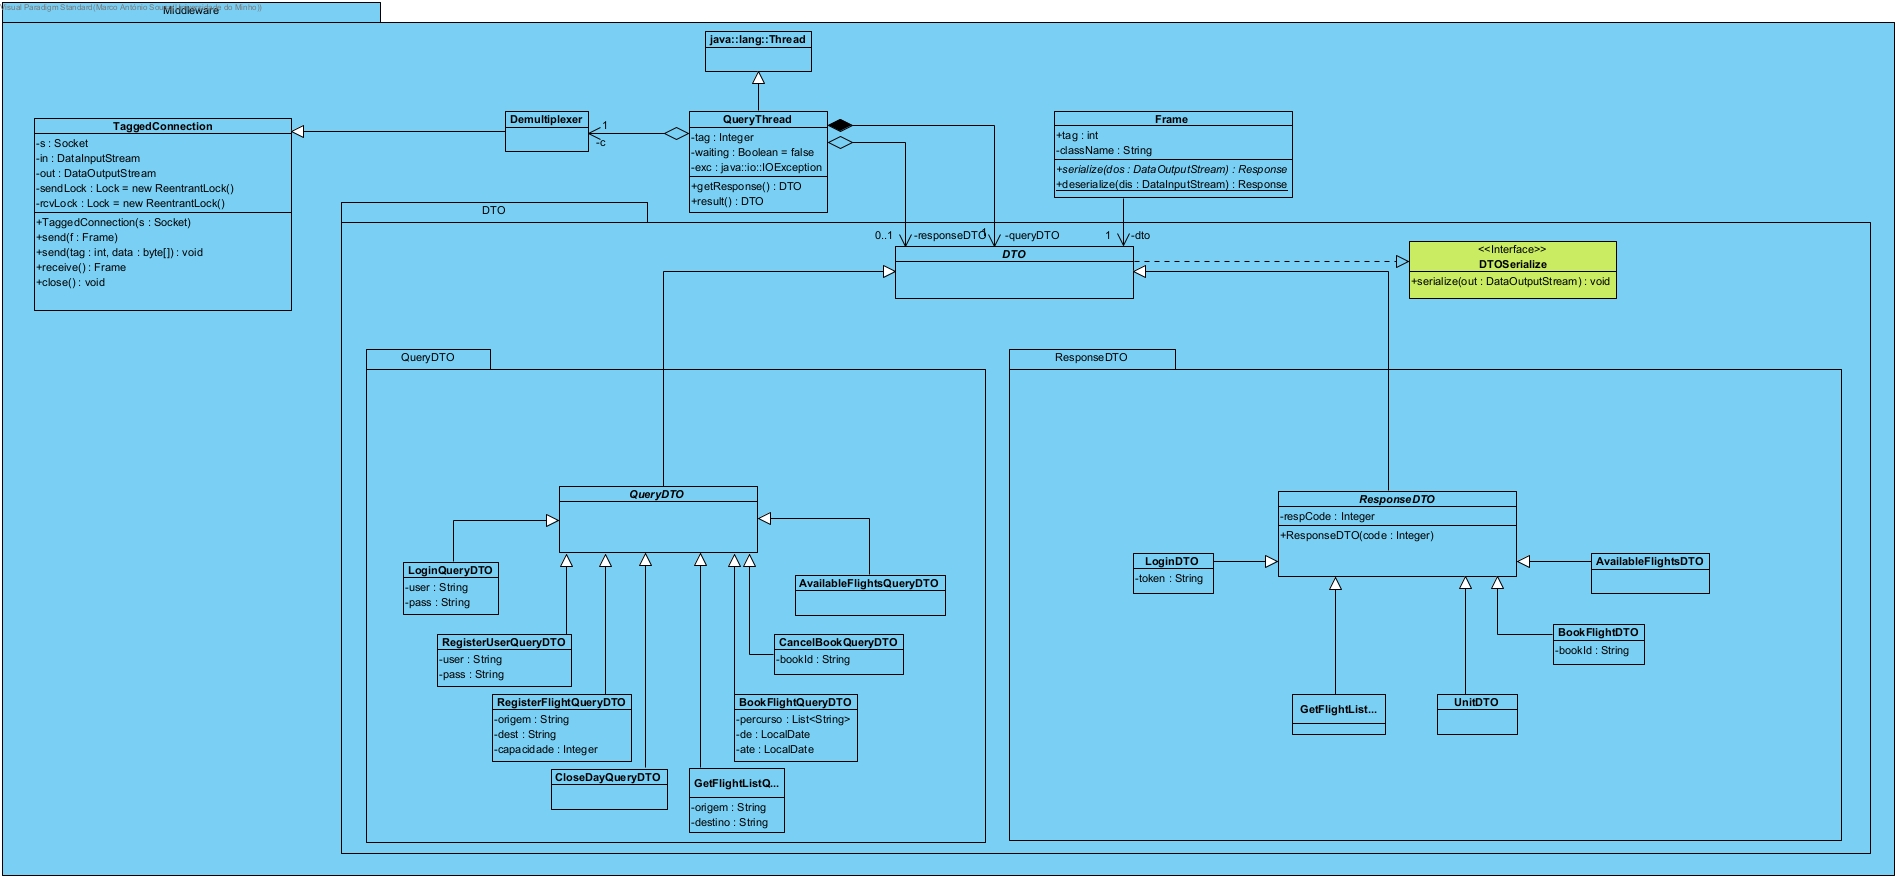
\includegraphics[width=\linewidth]{diagramas/MiddlewareClassDiagram.jpg}
    \caption{Diagrama de Classes - Middleware} \label{img:middleware}
\end{figure}
\end{landscape}

\begin{landscape}
\addsec{Anexo 4 - Diagrama de Classes do FlightManager (Servidor)}
\begin{figure}[!ht]
    \centering
    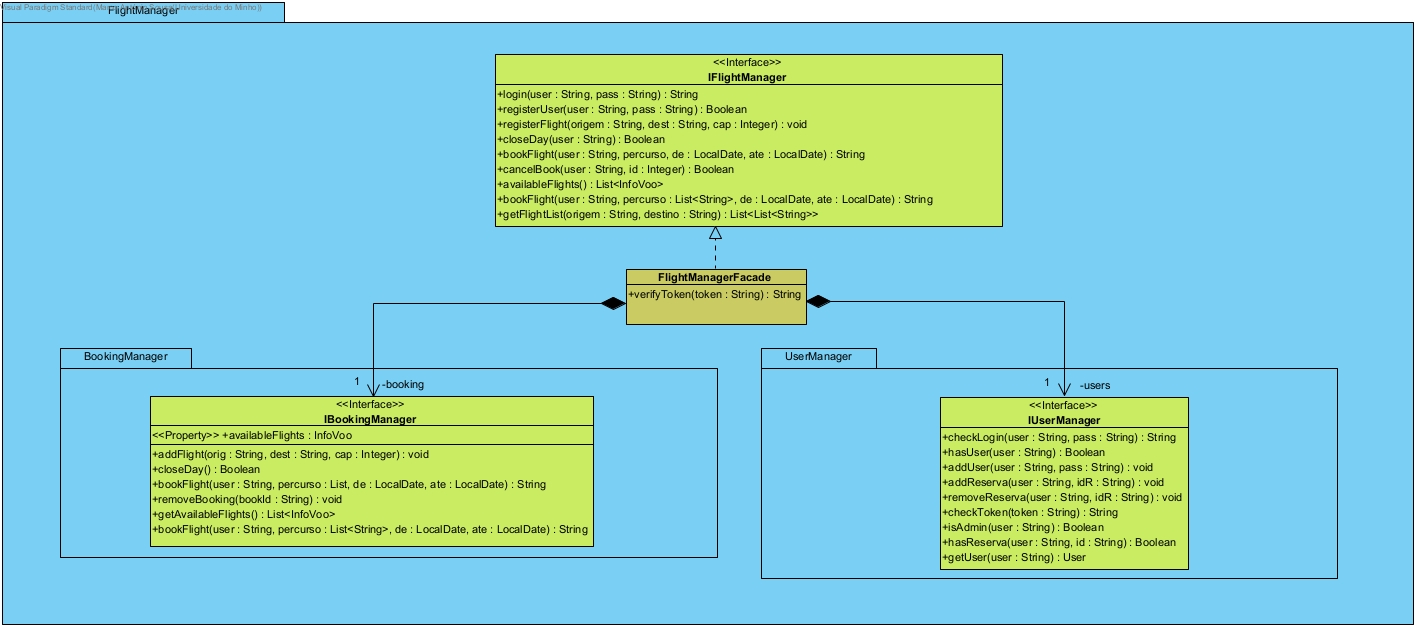
\includegraphics[width=\linewidth]{diagramas/FlightManager.jpg}
    \caption{Diagrama de Classes - FlightManager} \label{img:flight_manager}
\end{figure}
\end{landscape}
%==========================================================================
% END ANEXOS
%==========================================================================

\end{document}